\documentclass[twoside,leqno,twocolumn]{article}
\usepackage{ltexpprt}
% -- Grace inserted --
\usepackage{amssymb}
\usepackage{graphicx}
\usepackage{subfigure}
\usepackage{amsmath}
\usepackage{multirow}
\usepackage{mathrsfs}
\usepackage{algorithm}
\usepackage[noend]{algorithmic}
\usepackage[usenames,dvipsnames]{color}
\usepackage{tabularx,booktabs}
\usepackage{bm}
\usepackage{cite}
\newcommand{\Yuedit}[1]{{\color{magenta} #1}}
%\newcommand{\Yucomment}[1]{{\color{blue}{[Yu: #1]} }}
%\newcommand{\Yuremove}[1]{{\color{gray}{YuRemove: #1} }}
% -- Grace inserted end --

\begin{document}

\title{\Large Real-time Estimation of the Urban Air Quality with Mobile Sensor System}
\author{Yun Wang\\
Peking University\\
wangyun94@pku.edu.cn\\
\and
Lun Du\\
Peking University\\
dulun@pku.edu.cn\\
\and
Zhicong Lu\\
Peking University\\
phyluzhicong@pku.edu.cn\\
\and
Guojie Song\\
Peking University\\
gjsong@pku.edu.cn\\
\and
Zhanyuan Yu\\
Peking University\\
yuzhanyuan1995@gmail.com\\
%yu\underline{}zy@pku.edu.cn\\
\and
Mengfei Ruan\\
Beijing University of Technology\\
cynthia6639@sina.com\\
}
\maketitle

\begin{abstract} \small\baselineskip=9pt
Recently, real-time air quality estimation has attracted more and more attention from all over the world, which is convenient for our daily life. With the prevalence of mobile sensors, there is an increasingly available way to monitor the air quality with mobile sensors on vehicles, different from traditional expensive monitor stations. In this paper, taking advantage of air quality data from mobile sensors, we propose an real-time urban air quality estimation method based on the Gaussian Process Regression for air pollution of the unmonitored areas. In our model, we present two kinds of kernel functions to measure the distance among the spatio-temporal, climate and pollution features from periodicity and adjacency similarity, respectively. In order to meet the real-time demands, we propose a two-layer ensemble learning framework and apply KD-Tree on it to improve self-adaptivity and computational efficiency. We evaluate our model with real data from mobile sensor system located in Beijing, China. And the experiments show that our proposed model is superior to the state-of-art spatial regression methods in both precision and time performances.
\end{abstract}

\section{Introduction}
\noindent In recent years, air quality has attracted increasingly attention from all over the world. Serious surface-level air pollution are responsible for a range of diseases. Nowadays, air quality monitor stations have been built to inform people of air quality every hour in many cities. However, it is so expensive to establish and maintain air quality monitor stations which only provide sparse information about the spatial distribution of air pollutants. Due to the sparse observations from static stations, many existing methods are good at the coarse-grained estimation, not fine-grained in terms of time. \cite{Hsieh2015Inferring} \cite{Grover2015A}. However, compared to the coarse-grained estimation, real-time estimation is more significant to people's daily life to some extent\cite{Zhang2012Real}.
\begin{figure}[tbp]
\centerline{
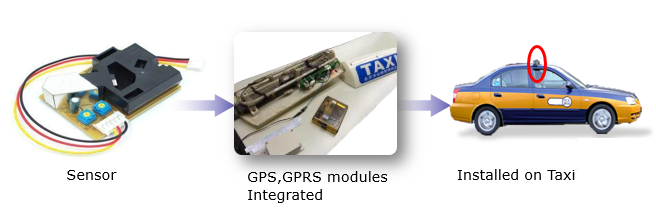
\includegraphics[width=0.9\linewidth]{pictures/equipment.png}
}
\caption{\label{fig:equipment}A mobile sensor for monitoring air quality located on the taxi}
\end{figure}

With the prevalence of available and affordable mobile sensors, there is an emerging way to monitor the air quality by the mobile sensors, which can provide abundant and fine-grained monitoring data for us. In this paper, the experiment data set is from the mobile sensor system located in Beijing which consists of 51 taxis equipped with mobile sensors to monitor the concentration of $PM_{2.5}$ (Figure \ref{fig:equipment}). The monitoring frequency is once every 30 seconds, generating about 35 thousands monitoring data every day. Especially, the spatio-temporal distribution of monitoring positions depend on the random positions of taxis in the city, which can be seen in Figure \ref{fig:Sampling}. The abundant data set gives us an opportunity to do real-time air quality estimation.

There are some challenges to do real-time estimation with monitoring data from mobile sensors. The first challenge is the contradiction between the huge amount of data and the high demand time performance of real-time application. The second challenge is to improve the self-adaptivity of the real-time estimation model. The third challenge is the non-uniform property of the spatio-temporal distribution of monitoring data. If we just use the latest observations to do the real-time estimation, it's difficult to get reliable results on these areas with sparse observations. Therefore, how to make full use of historical information and diffusion of air pollutants is also a challenge.

To improve the time performance, we apply enhanced KD-tree to organize the original data into multiple homogeneous data sets and train each individual learner with these data set. And then the estimations from these individual learners can be integrated based on ensemble learning. In order to enhance the self-adaptability of model, we propose a two-layer self-adaptivity framework. Besides, the pollution of a region depends on its own land use and the dispersion from other places. To solve the problem of non-uniform spatio-temporal distribution of data, a new data sampling mechanism is proposed to select more related data for the query point, which combines the principle of pollutants generation.

The main contribution of this paper can be summarized as follows:
\begin{enumerate}
 \item We present a Real-time Ensemble Estimation Model (REEM) based on Gaussian Process Regression, which takes advantage of air quality observations from mobile sensors located on the taxis;
 \item We introduce two kinds of kernel functions to discovery the periodic and adjacent similarity patterns from the spatio-temporal, climate and pollution features, respectively.
 \item We propose a data filter mechanism to obtain more related observations for a certain query point.
 \item We present a two-layer ensemble learning framework and apply KD-tree to improve self-adaptivity and computational efficiency;
 \item Experiments show that our proposed model outperforms the traditional spatial regression methods in both precision and time cost.
\end{enumerate}
The rest of the paper is organized as follows: We next conclude related work. In section of preliminaries, we define our problems and review the Gaussian Process Regression. We describe the technical details of our approach in section 4. In section 5, the results of experiments on real-world data can be found, and we also evaluate it against state-of-art approaches. Finally, we summarize our work and discuss future work in section 6.

\section{Related Work}
In general, there are two kinds of main techniques for real-time air quality estimation \cite{Waylang}:

Deterministic model, which follows the principle of atmosphere dynamics, simulates the transport and diffusion of atmospheric particulate matters with a series of physical and chemical equations. Generally, these models are sophisticated and good at coarse-grained estimation. \cite{zhang2008online}\cite{Pfender2006Use}

Statistical approaches: Some of the existing real-time estimation models based on measurements are too simple to lead to high accuracy such as the Inverse Distance Weighted(IDW), where the distances between query points and sample points are weighted average. Some have high computational complexity which cannot adapt the demand of real time when dealing with large amounts of data, e.g. Kriging \cite{odeh1995further} or standard Gaussian Process Regression(GPR) \cite{rasmussen2006gaussian}, whose computation complexity is $O(N^3)$ with a set of N training set.
In recent years, there have been some state-of-art models, which found the trade-off between accuracy and computational complexity. \cite{guizilini2015nonparametric} introduces a method, a Nonparametric Online Model(NOM), for the continuous online prediction of particulate matters in the air given sparse sensor information, applying sub-sampling based on frequency analysis to reduce the computational complexity.  \cite{Nguyen2008Local} proposes Local Gaussian Process Regression(LGP) for real-time estimation. But these methods are based on sparse data sets mostly from air quality monitor stations.

The method of collecting data by mobile sensors has attained much more attention recently due to its low cost, portability and easy maintenance \cite{Hasenfratz2015Deriving}. The mobile sensor for air quality monitoring was originally installed on public transportation which had a relatively fixed route\cite{Devarakonda2013Real}\cite{Jutzeler2014A}. And then, more and more private cars are installed with mobile sensors, which can collect air quality data in a broader area. As the sensors become smaller, there is a trend that handhold mobile devices become a tool for data collection.

\section{Preliminaries}
Air quality estimation is essentially a regression problem. As for a set of N air quality observations $T=\{\bm{X_i}, y_i\}^N_{i=1}$, $\bm{x_i}=(x_i^{spatio}, x_i^{time}, x_i^{weather})$ contains space, time and weather components and $y_i$ is the concentration of pollutants at query points. Our goal is to learn a transformation function $f(\bm{x_i})$ mapping the inputs $\bm{x_i}$ to the pollutant value, given $y_i = f(\bm{x_i})+\varepsilon$, where the $\varepsilon$ usually represents noisy.

Gaussian Process extends multivariate Gaussian distribution to infinite dimensionality, determined by the mean function $m(\bm{x})$ and the kernel function $k(\bm{x},\bm{x}')$. We set the mean function $m(\bm{x})$ as zero function and note that:
\begin{equation}
 f(\bm{x}) \sim GP(0, k(\bm{x}, \bm{x}'))
\end{equation}
the joint distribution of observed values and predicted value for a query point $x_*$ is given by:
\begin{equation}
    \left[ {\begin{matrix}
	  	y\\
	  	y_*
	 \end{matrix}} \right]
   \sim
   {\rm N}(0,\left[ {\begin{matrix}
	  {K(X,X) + \sigma _n^2{I_n}}&{K(X,{x_*})}\\
	  {K({x_*},X)}&{K({x_*},{x_*})}
	 \end{matrix}} \right])
\end{equation}
Following the Bayesian paradigm, we can get the posterior probability distribution of $y_*$:
%\begin{equation}
\[
 y_*|x_*,X,y \sim N(\bar{f}(x_*), \mathbb{V}[f(x_*)])
\]
%\end{equation}
where

\[
 \bar{f}(x_*)=K(x_*, X)[K(X,X)+\sigma_n^2\bm{I}]y
\]
\begin{equation}
\begin{aligned}
 \mathbb{V}[f(x_*)]&=K(x_*, x_*) \\ \notag
 -&K(x_*, X)(K(X,X)+\sigma_n^2\bm{I})^{-1}K(x_*, X)
\end{aligned}
\end{equation}
From the above formulas, we can get the best estimation $y_*=\bar{f}(x_*)$.

The hyper-parameters of Gaussian Process are $\theta=[\theta_k, \sigma_n]$, where the $\theta_k$ is the kernel function parameter and the $\sigma_n$ is the noise parameters. We can get the optimal value for a certain data set by maximizing the log marginal likelihood(Equation \ref{equ:likehood}) using common optimization algorithms.
\begin{equation}
\label{equ:likehood}
\bm{p}(y|X,\theta)=-\frac{1}{2}y^TK^{-1}y-\frac{1}{2}log|K|-\frac{n}{2}log2\pi
\end{equation}

Thus, it can be seen that the main limitation of GPR is the computational complexity of $O(n^3)$ with n training examples. Especially, GPR is not appropriate for real-time estimation when training large amounts of data.

%--- luke

\section{Real-Time Ensemble Estimation Model}
In this section, we present a Real-time Ensemble Estimation Model(REEM) for air quality estimation. First of all, we propose a data organizing method based on the KD Tree, as well as a training method of individual learner based on gaussian process. Next, we put forward a data filter mechanism and an ensemble estimation method based on frequency analysis. Finally, we present a two-layer self-adaptivity framework in a real-time environment.

\subsection{Partition and Training based on KD-Tree}
As discussed before, the data sampling frequency of mobile sensor is high for about 2 times per minute generating a large training set. However, the common drawback of standard GPR is time-consuming, which makes it hard to adjust hyper-parameters immediately with up-to-date data.  In order to overcome the problem, we divide the data based on KD-Tree and train several individual learners based on GPR using an ensemble learning method.

\subsubsection{Data Partition based on KD-Tree}
The KD-Tree is a balanced binary tree which can be used to partition a set of data with arbitrary dimensions efficiently.  Each node contains a subset of the data. And in a certain layer, the data of each node is divided according to the distance of a certain dimension. Thus, the nodes located at deep layers contain subsets of adjacent data.

In common spatial interpolation problem, it is a basic assumption that the output should be similar if two samples are close to each other in spatial. In air quality estimation problem, we assume that sampling nodes with similar weather  properties are also supposed to have similar outputs. Thus we regard the longitude, the latitude and the weather properties of the sampling nodes as the KD-Tree partition measure. Figure  \ref{fig:KD-Tree} is a partition example of KD-tree structure in which each cuboid is a tree node and each small cube represents a data point in feature space.

\begin{figure}[htbp]
\small
\centering{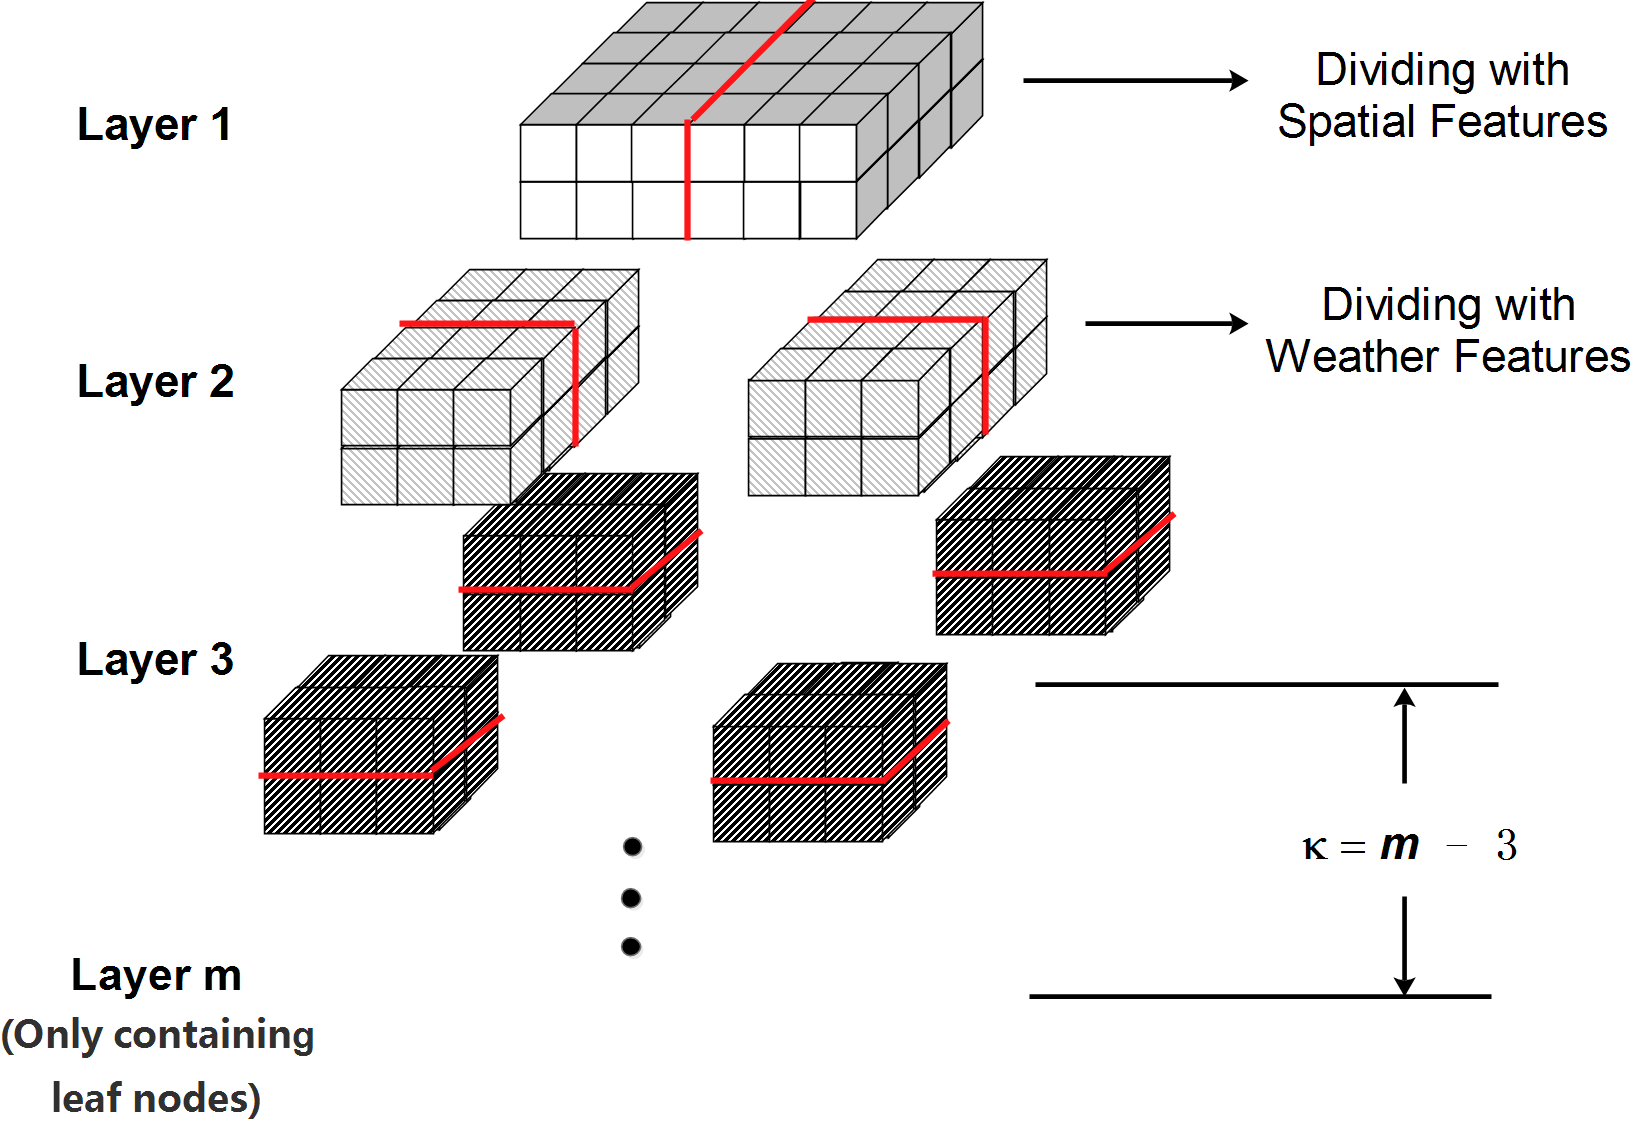
\includegraphics[width=0.45\textwidth] {pictures/kd-tree.png} }

\caption{A Sample of KD-Tree Structure}
\label{fig:KD-Tree}
\end{figure}

In the ensemble learning field, the result of prediction or classification is better when each individual learner contains as much homogeneous data as possible. Therefore, we select data subsets from parts of non-leaf nodes in the KD-Tree as the training sets of individual learners. Specifically, we set the threshold as $\kappa\in[1,d_{tree})$, where $d_{tree}$ is depth of the KD-Tree, and select the $(d_{tree}-\kappa)$ th layer as the divided layer. And figure \ref{fig:KD-Tree} illustrates a example of $\kappa$ selection.

As KD-tree is balanced binary tree, the number and scale of data subset can be decided to make sure that the size of datasets is basically the same. That is:
\[
	m=2^{d_{tree} - \kappa}
\]
\[
		\forall i\in[1,m],\quad  d_{tree} - \kappa + 2^{\kappa-2}<|S_i| < d_{tree} - \kappa + 2^{\kappa}.
\]
where $m$ is the number of training subsets and $S_i$ is the $i$ th training subset. In this way, we can avoid the problem of uneven data quantity in each individual learner caused by uneven distribution of the data. In addition, we enhance the kd-tree with additional information in the $\kappa$ th layer including the time features of data and hyper-parameters after training.

 \subsubsection{Individual Models Training}
In each training subset, we train an individual GP model that allows to reflect the prior knowledge of the problem by designing kernel function.
%Kernel selection
Based on the spatio-temporal adjacency simularity and time periodicity of data, our kernel is:
\begin{equation}
\begin{split}
\label{equ:kernelF}
k_f(x_*, x) = &\sigma_{w}^{2}\exp\{-\frac{1}{2}D^T_{wheather}MD_{weather}\}\times\\
	&\sigma_{s}^{2}\exp\{\frac{||D_{spatio}||^2}{l_s}\} \times k_{t}(||D_{time}||)\\
\end{split}	
\end{equation}
%\begin{equation}
%\label{equ:kernel_t}
%k_{SM}(\tau) = \sum^A_{a=1} \omega_a^2\exp\{-2\pi^2\tau^2\varphi_a^2\}\cos(2\pi\tau\mu_a)
%\end{equation}
\begin{equation}
\begin{split}
\label{equ:kernel_t}
k_{t}(x_*, x) &= \sum_{a=1}^{\bm{A}} k_t^a(x_*, x) \\
&=\sum_{a=1}^{\bm{A}} w_a^2 exp\{-2 \pi^2 r^2 \sigma_a^2\}cos(2\pi r \mu_a)
\end{split}
\end{equation}
where $D_i = x_i - x'_i, ~ M=diag(\bm{l_w})$. Formula \ref{equ:kernel_t} is the kernel function of time $r = x_*^{time}-x^{time}$, which is a spectral mixture (SM) kernel \cite{Wilson2013Gaussian},
and is an expressive basis for approximating any stationary covariance functions to arbitrary precision. $\bm{A}$ is the number of different frequencies we select. According to our experiments, $\bm{A} = 3~or~ 5$ is enough to capture the short and medium-scale periodicity in the data. The frequencies are initialized from a uniform distribution from 0 to Nyquist frequency considering the sensitivity of the SM kernel on small data sets.

As can be seen, the value of kernel function reflects the distance of samples after mapping. Considering the Gaussian noise in our observations, the final kernel function is:
\begin{equation}
\bm{K}(\bm{X},\bm{X})=\bm{K_f}(\bm{X},\bm{X'})+\sigma_n^2\bm{I}
\end{equation}
We define a GPR model under the air quality estimation situation, which involves the following hyper-parameters:
\[
\bm{\theta}=(\sigma_s^2, \sigma_w^2, l_s, l_w, \bm{\omega}, \bm{\varphi}, \bm{\mu}, \sigma_n^2).
\]

\subsection{Data Filter and Estimation}
For a given query point, we first apply a data filter mechanism to refine the estimation data set, and then obtain the final estimation output based on ensemble learning.
\subsubsection{Data Filter Mechanism}
The figure \ref{fig:Sampling} illustrates the non-uniform properties of the spatio-temporal distribution of mobile monitoring data. Thus, it is hard to obtain reliable estimations with latest monitoring data, especially on those areas with sparse observations. This can be solved by training model with history monitoring data, in this way our model can use the discovered pattern to accomodate various distributions of observations. In order to reduce the computation complexity of large amounts of history monitoring data, we introduce a data filter mechanism to refine the training data set for each query point.

As mentioned before, the data with similar space and weather features can be organized into the same individual learner through the enhanced KD-tree. The reason why we don't choose the time feature as a standard to construct KD-tree is that the adjacency similarity of the data guaranteed by KD-tree can not express the periodicity of the time feature. Therefore, we apply filter mechanism to refine the training data of each individual learners in order to discover the periodicity of time easily in our model. The filter rule can be defined as follows:

\begin{align}
\{ \bm{X}, y \}_{x_*}^a = \{~ (x, y&)_n ~ | \mod(||x_*^{(t)}, x_n^{(t)}||, \frac{1}{\mu_a}) < \frac{\delta}{\mu_a})~\} \label{equ:filteringrule} \\
%\{ \bm{X}, y \}_{x_*}^a = \{ ~(x, y)_n ~&|~ k_t^a(x_*, x_n) > \delta \sum_{i=1}^N k_t^a(x_*, x_i) ~ \}_N \label{equ:filteringrule} \\
S_{x_*} =& \{ X, y\}_{x_*} = \bigcup_{a=1}^A\{x, y\}_{x_*}^a \notag
\end{align}
As a multiplier of our kernel function $k(x_*, x)$, if $k_t(x_*, x)$ is tiny,  $k(x_*, x)$ is close to 0(formula \ref{equ:kernelF}). And the $K_t(x_*, x)$ is positively related to the phase difference(i.e.$\mod(||x_*^{(t)}, x_n^{(t)}||, \frac{1}{\mu_a})$). Thus we can set a threshold and remove all data which falls below the threshold. Here $\delta$ is a constant and . $\{\bm{X}, y\}_{x_*}^a$ (Formula \ref{equ:filteringrule}) means the most correlated data set in a certain frequency $\bm{a}$ for the query point $x_*$. And $S_{x_*}$ is called the estimation set for the query point $x_*$.

\begin{figure}[htbp]
\small
\centering{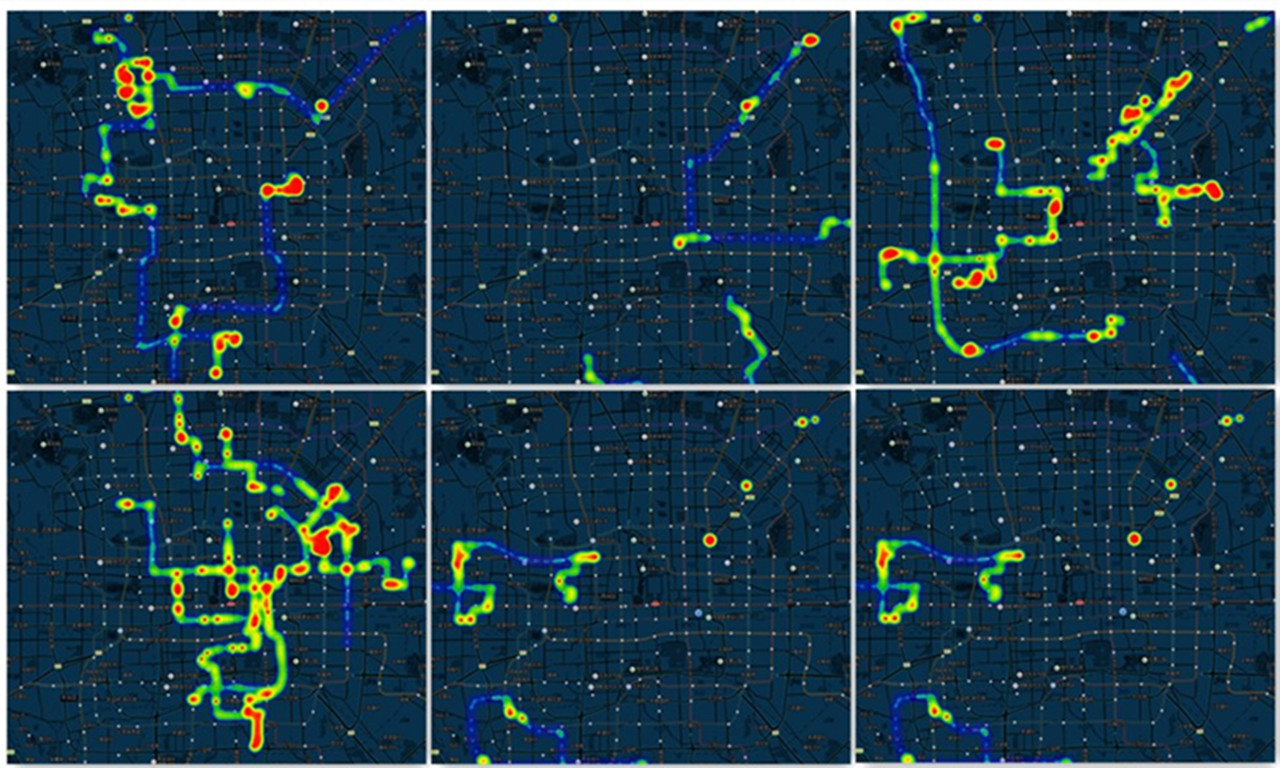
\includegraphics[width=0.43\textwidth] {pictures/Sampling.png} }

\caption{Monitoring Distributions at Different Periods in One Day}
\label{fig:Sampling}
\end{figure}


\subsubsection{Ensemble and Estimation}
The extent of pollution in a region is determined by the cumulation effect and the propagation effect. The cumulation effect of pollutants is related to the land use of a region and has its own regularity and periodicity in terms of time.
And the weather-driven and distance-driven propagation effect corresponds to the spread of pollutants with obvious adjacent similarity.

The estimation model based on enhanced KD-tree ensures the adjacency similarity of the data sets for each individual learner in the weather and space features. Thus, for a given query point $x_*$, the nearest individual learner $L_{nearest}$ can be found with enhanced KD-tree. Data filter mechanism should be applied to the data set of $L_{nearest}$ to refine the most correlated data as the estimation data set, which reflects the cumulation effect of pollutants(Formula \ref{equ:filteringrule}). For other individual learners of our model, we choose the up-to-date monitoring data as their estimation data set, which reflects the propagation of pollutants. Finally, the estimation value $y_*$ is performed using weighted averaging over $m$ individual predictions $y_*^{(i)}$. After the formal definitions, we can train each subset based on the GPR method as discussed above:
\begin{equation}
y_*=\frac{\sum_{i=1}^mw_iy^{(i)}_*}{\sum_{i=1}^mw_i}
\end{equation}
we use the average results of the kernel function $K(X, x_*)$ in each estimation data set as the weight of ensemble to further improve the computation efficiency of prediction and train.
 \begin{equation}
 w_i =  mean(\bm{K}(x_*,\bm{X^{(i)}}))
 \end{equation}
where $\bm{X^{(i)}}$ is the estimation data set for the $i$ th individual learner. The details can be seen in Algorithm \ref{alg:prediction}.
\begin{algorithm}[htb]
\caption{Ensemble Prediction}
\label{alg:prediction}
\begin{algorithmic}[1]
\REQUIRE ~~\\
the query point $x^*$ \\
the origin data set $S$
\STATE $S_{nearest} = FindNearestLearner(S, x^*)$
\STATE $S_{estimation}^* = DataFilteringMachanism(S_{nearest})$
\STATE $y^*_{nearest} = GP(S_{nearest}^*)$
\FOR{$ S_i \in S-S_{nearest}$}
    \STATE $S_i^* = FindLatestData(S_i)$
    \STATE $y_*^{(i)} = GP(S_i^*)$
\ENDFOR
\STATE $y_*=\frac{\sum_{i=1}^m mean(\bm{K}(*,\bm{X^{(i)}}))_i * y^{(i)}_*}{\sum_{i=1}^m mean(\bm{K}(*,\bm{X^{(i)}}))}$
\STATE Output($y_*$)
\end{algorithmic}
\end{algorithm}


\subsection{Two-Layer Self-Adaptivity Framework}
In order to improve the self-adaptivity of model in the real-time environment, we need to update the model in accordance with the up-to-date data without delay. The standard GPR uses new data to update the covariance matrix by calculating the inverse of matrix again, whose time complexity is O($n^3$) and can hardly match the real-time request. Besides, when the time span is large, the hyper-parameters need to be trained again to adjust to the change of the environment(e.g climate change and periodicity change of time). However, the training of standard GPR is time-consuming, which makes it hard to adjust hyper-parameters in time. In this paper, based on the high efficiency of KD-Tree insertion and deletion, we design a two-layer updating framework, which applies different strategies to update the model in different lengths of time windows.

The figure \ref{fig:AF} shows our self-adaption framework. Each small rectangle represents the data in a time slice. $T_l$ and $T_s$ denote the lengths of two time windows respectively. $T_l$ is a threshold we set and $T_s$ is a variable affected by the real-time estimation error and the time after the last training. In the framework, the data in $T_l$ time window is used for training hyper-parameters and constructing KD-Tree, i.e.
\begin{equation}
	\{\bm{X}, \bm{y}\}_{training}^h = \{(\bm{x}, y)~|~ x^{time} \in [h, h + T_l] \}
\end{equation}
where $h$ is current time slice.
%insert picture(eps) (using command "convert name.png name.eps")
\begin{figure}[htbp]
\small
\centering{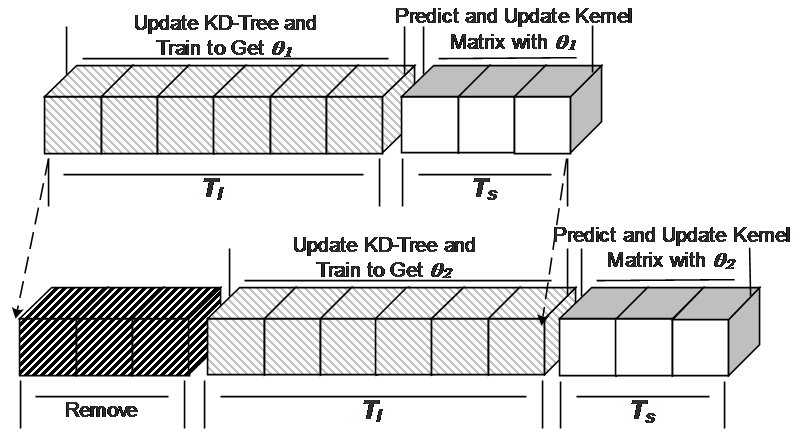
\includegraphics[width=0.4\textwidth] {pictures/Framework.png} }

\caption{Self-Adaption Framework}
\label{fig:AF}
\end{figure}

In our framework, we do not adjust hyper-parameters in every time slice because training for every 30 seconds leads to a expensive time cost. After each training, we update the training set and re-train the model after $T_s$ time slices. $T_s$ is determined by the equation \ref{Eq:Ts_set}

\begin{align}
    T_s &= T \notag  \quad  s.t. \notag \\
    \forall t \in [0, T), ~& \sum_{p\in P(t)}t \times Err^{(p)} - \theta \times |P(t)| \times T_l < 0 \label{Eq:Ts_set}\\
     \sum_{p\in P(t)}T & \times Err^{(p)} - \theta \times |P(t)| \times T_l \geq 0 \notag
\end{align}
where $Err^{(p)}$ indicates the relative error between the $p$-th monitoring  and estimation value; $T$ is the number of time slices after the last training; $P(t)$ is the monitoring values set we select at the $t$-th time slice and $\theta$ is a threshold drawn from the experiment. It is easy to see from the formulation above. When average relative error in a time period and the time after the last training are both relatively large, it is time to re-train the model and update the KD-Tree.

Moreover, in a relative short time period, the hyper-parameters will only have little changes because of the temporal adjacency simularity of data. Thus we use the same hyper-parameter for estimation and adjust the model adaptively through updating the training subsets as well as recalculating kernel matrices in the $T_s$ length of time slice after each training, i.e. for a  new  sample $[\bm{x_{new}}, y_{new}]$
\begin{equation}
	\begin{split}
	\bm{K^{(i)}_{new}} = &\bm{K}([\bm{X^{(i)}}, \bm{x_{new}}], [\bm{X^{(i)}}, \bm{x_{new}}]), \bf{if} ~ \bm{x_{new}} \in \bm{S^{(i)}}. \\
	\end{split}
\end{equation}

When the time reaches $T_s$ after training, we slide the training time window and remove stale samples $\bm{X_{remove}}$ from KD-Tree.
\[
	{\bm{X_{remove}}} = \{\bm{x}~|~ x^{time} \in [h - T_l - T_s, h - T_l]\}
\]
And the new samples $\bm{X_{add}}$ is added to KD-Tree.
\[
	{\bm{X_{add}}} = \{\bm{x}~|~ x^{time} \in [h - T_s, h]\}
\]
Due to the nature of KD-Tree, the efficiency of deletion and insertion is very high, and the tree structure can be adjusted adaptively through the rotation of nodes to ensure the homogeneity of the data in each subset. And then each training subset will be trained again. The overall framework of the model is detailed in algorithm \ref{alg:MCT}.


\begin{algorithm}[htb]
\caption{Model Update and Prediction Framework} \label{alg:MCT}
\begin{algorithmic}[1]
\REQUIRE ~~\\
Initial training set, $\{\bm{X}, \bm{y}\}$\\
Threshold, $\kappa, T_l, T_s$
\STATE $Tree= Build(\bm{X})$
\STATE $\bm{S} = GetSubsets(Tree, \kappa)$
\FOR{$\bm{S^{(i)}} \in \bm{S}$}
   \STATE $\bm{K^{(i)}}=GP(\bm{S^{(i)}})$
\ENDFOR

\WHILE{$HaveNextTimeslice()$}
    \STATE $\{\bm{X_{new}}, \bm{y_{new}}\}=GetNewData()$
     \IF {$IsNeedRetrain(\{\bm{X_{new}}, \bm{y_{new}}\})$}
        \STATE $\bm{Tree}.Update()$;
        \FOR{$\bm{S^{(i)}} \in \bm{S}$}
              \STATE $\bm{K^{(i)}}=GP(\bm{S^{(i)}})$
        \ENDFOR
     \ELSE
        \FOR{$\{\bm{x_i}, y_i\} \in \{\bm{X_{new}}, \bm{y_{new}} \}$}
           \STATE $id = Tree.find(\{\bm{x_i}, y_i\})$
           \STATE $\bm{K^{(id)}} = \bm{K}([\bm{X}, \bm{x_{i}}], [\bm{X}, \bm{x_{i}}])$
            \STATE $\bm{y^{(id)}}=\bm{y^{(id)}} + y_i$
         \ENDFOR
      \ENDIF

    \FOR {$\bm{x_*} \in \bm{S_w}$}
       \STATE $y_* = EnsemblePrediction(\bm{x_*}, \bm{S})$
       \STATE Output(${\bm{x_*}, y_*}$)
    \ENDFOR
\ENDWHILE

\end{algorithmic}
\end{algorithm}


\subsection{Complexity Analysis}
In the training process, the time complexity of each iteration is O ($k^3$), where $k=\frac{n}m$ using the maximum likelihood method with $m$ training subsets. And for all subsets, the total complexity of the iteration is O ($k^3\times m$).  The computational efficiency is greatly improved, compared to the traditional GPR with O ($n^3$) time complexity. In addition, the time complexity of estimation is O($n$), so it can be applied to the real-time scenarios.

In the adaptive updating process of the model, the time complexity of KD-Tree insertion and deletion is O ($\log (n) $) which can be negligible. And the time complexity of recalculating kernel matrices is O ($k^3\times m$), which also has a greater improvement than the time complexity O($n^3$) of traditional GPR .

%--end luke --

\section{Experiments}
In this section, our model, Real-time Ensemble Estimation Model(\emph{REEM}), are evaluated using the climate data and the air quality data from mobile sensor system(Figure.\ref{fig:display}). The performance of \emph{REEM} is compared with the state-of-art interpolation models, e.g. standard \emph{GPR}, \emph{Kriging}, \emph{IDW} and \emph{LGP}. The goal of models is to estimate the concentration of $PM_{2.5}$ at any given location.
\begin{figure}[!htb]
\centerline{
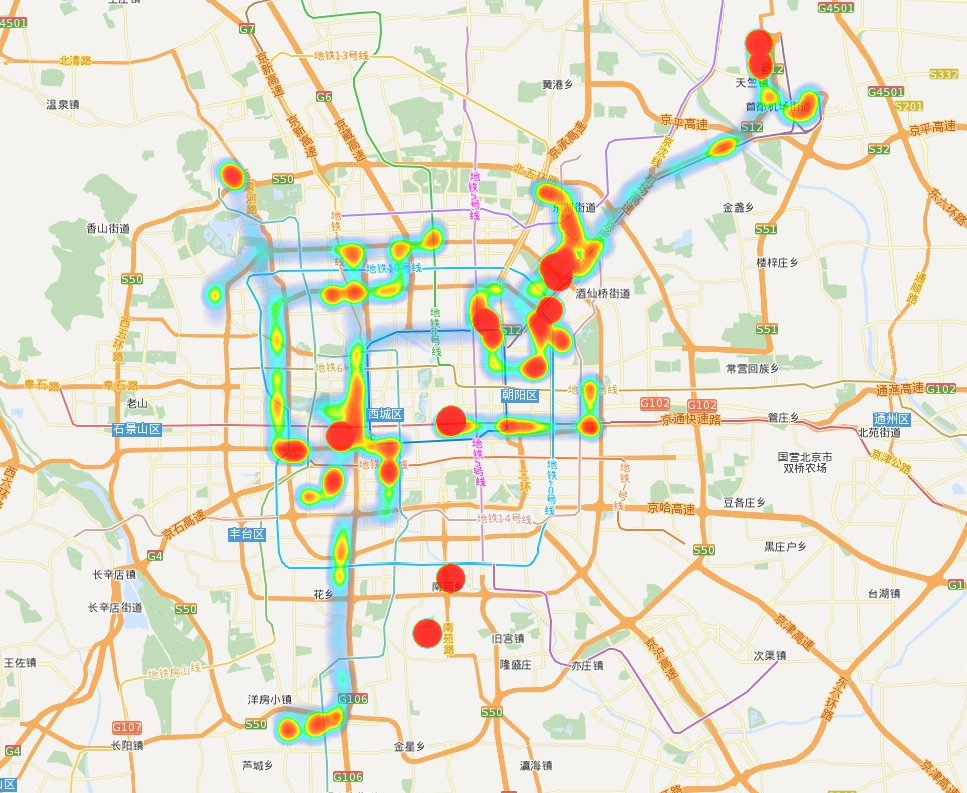
\includegraphics[width=0.68\linewidth]{pictures/display.png}
}
\caption{\label{fig:display}An real-time estimation result in Beijing at a certain time}
\end{figure}
\subsection{Data Set from Mobile Sensor System}
Our data set is from June 1st, 2015 to September 29th of totally 121 days, whose data sampling frequency is high for about 2 times per minute. The monitoring data is comprised of the sampling time, the concentration of $PM_{2.5}$, longitude and latitude. During this period, there are 51 mobile devices collecting data on road, while only several devices work at the same time. The number of records per day in June are shown in Figure \ref{fig:perday}, where the number is considerable and relatively stable. We also make an experiment to get the distribution of the number of records at every timestamp during one day. As shown in Figure \ref{fig:oneday}, the amount of records at different times fluctuates greatly, which is a challenge to real-time model.
\begin{figure}[!htb]
\centerline{
\subfigure{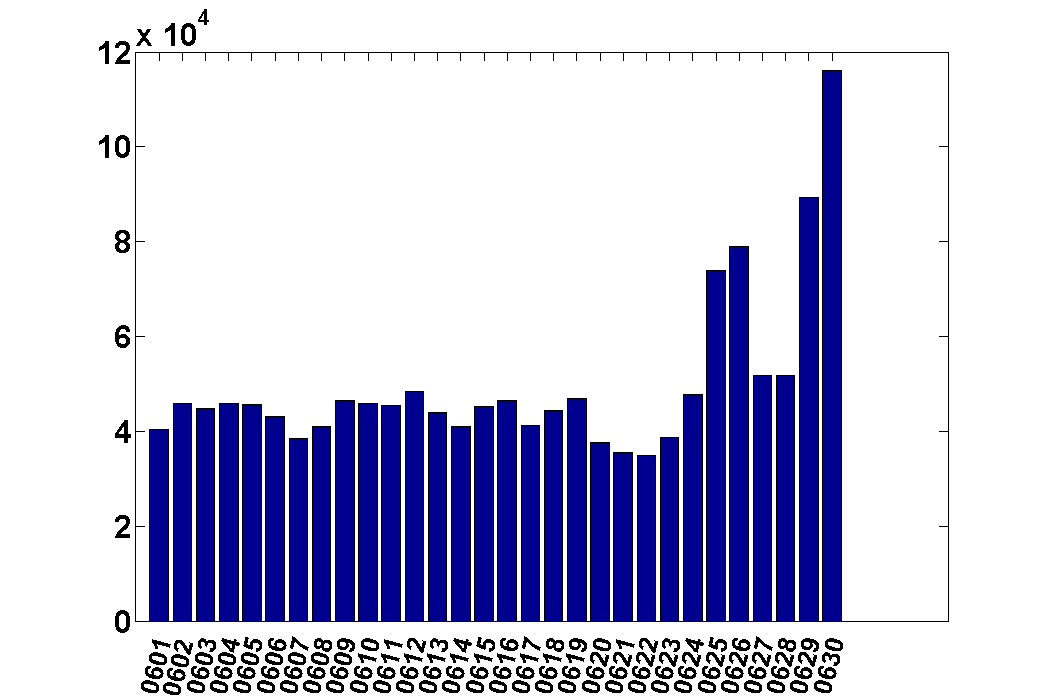
\includegraphics[width=0.49\linewidth]{pictures/recordsPerday.png}\label{fig:perday}}
\subfigure{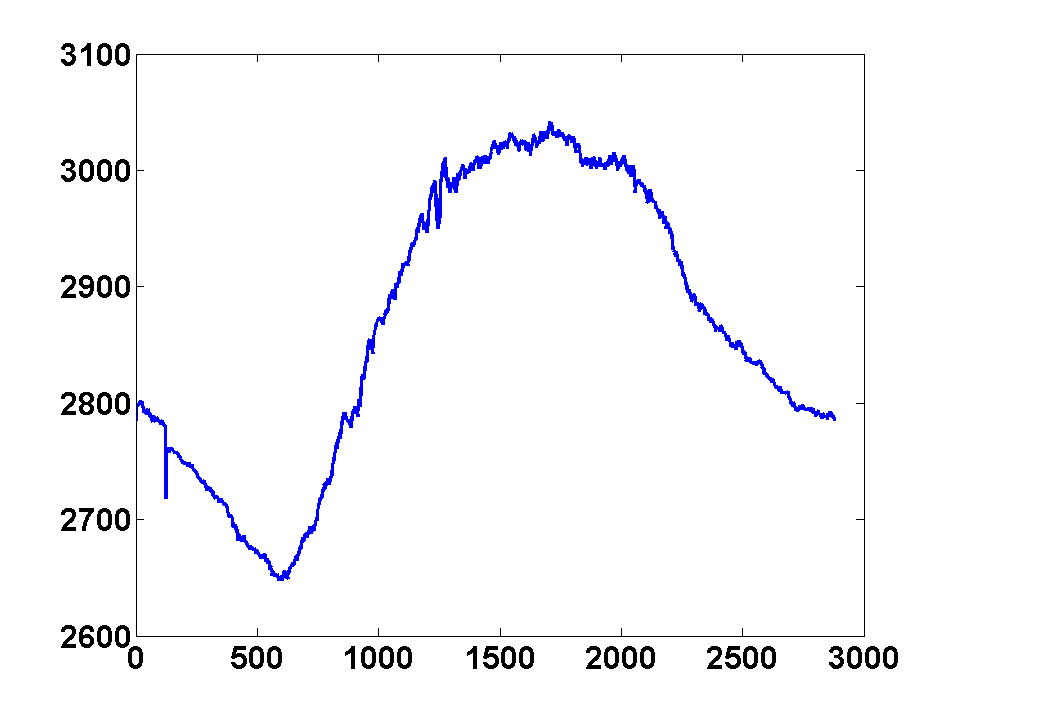
\includegraphics[width=0.49\linewidth]{pictures/recordsOneday.png}\label{fig:oneday}}
}
\caption{\label{fig:recordsPerday}Left:The number of records collected by mobile sensors per day in June. The horizontal coordinate x represents date, the format like '06XX' means XX days in June; the vertical coordinate y is the sampling volume; Right: The distribution of the number of records collected by mobile sensors at every timestamp during one day. The vertical coordinate y represents quantity of records; the horizontal coordinate x is timestamp, which of time interval is 30s}
\end{figure}

Based on the aforementioned analysis, we need to verify the validity and feasibility of models under different sampling densities.
%
\subsection{Kernel Selection}
%The Mean Average Error(\emph{MAE}) of the evaluation on different variables combinations is presented in Table\ref{tab:kCombination}. The performance of spatial feature is good. Additionally, the great improvement generated by the incorporation of time feature, which is in line with our conclusion that mobile data has strong spatio-temporal adjacent similarity. As well as the improvement generated by the inclusion of all of them. So, the input features we choose for our model consist of time, longitude, latitude, temperature, rain, pressure, humidity.
%
%\begin{table}[!ht]
%\footnotesize
%\caption{The comparison of evaluation on different variables combinations}
%\label{tab:kCombination}
%\def\tabblank{\hspace*{10mm}}
%\renewcommand{\multirowsetup}{\centering}
%\begin{tabularx}{0.5\textwidth}
%{@{\tabblank}@{\extracolsep{\fill}}lccp{100mm}@{\tabblank}}
%\toprule
%  Feature & MAE \\\hline
%  $K_{spatio}$ & 9.81 \\
%  $K_{time}$ & 32.40 \\
%  $K_{weather}$ & 19.52 \\
%  $K_{weather}+K_{time}$ & 16.87 \\
%  $K_{spatio}+K_{weather}$ & 10.67 \\
%  $K_{spatio}+K_{time}$ & 8.87 \\
%  $K_{spatio}+K_{time}+K_{weather}$ & 7.69 \\
%\bottomrule
%\end{tabularx}
%\end{table}
%
\subsection{$\kappa$ Selection}
In the selection experiment of $\kappa$, we choose 10000 training set and 3000 cross validation set. As shown in Figure \ref{fig:kappa}, The experimental results show that with the increase of K, the training time is positively correlated with K, which is because K determines the sample size of each individual learner, and the training time complexity is $O(n^3)$. As for RMSE, it shows a downward trend before increase. This is because the individual learner can be effective only if it ensures a certain amount of training samples. However, when the sample size is too huge, the homogeneity of the sample set divided into each individual learner will be weakened, resulting in decreased learning efficiency. According to these results, selecting $\kappa$ as 9 or 10 can produce better results.

\begin{figure}[!htb]
\centerline{
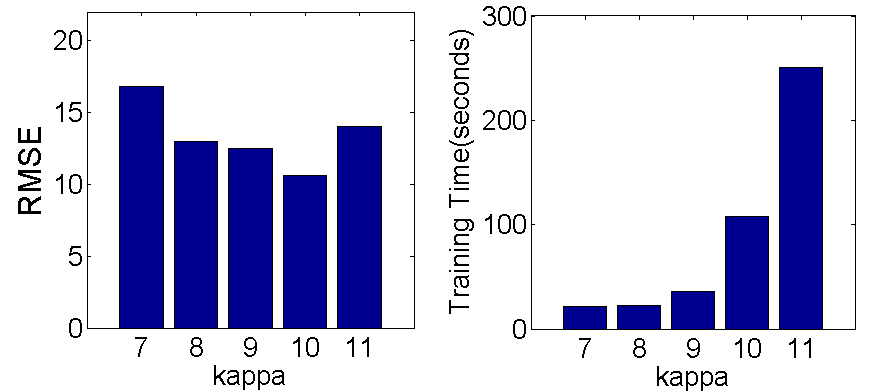
\includegraphics[width=0.9\linewidth]{pictures/kappa.png}
}
\caption{\label{fig:kappa}the experiment results at different $\kappa$}
\end{figure}
\subsection{Accuracy Comparison}
%Fig.\ref{fig:performance} shows the Logarithm Root Mean Square Error(\emph{LRMSE}) of evaluation on the test set for each size training set. As we can see from Fig.\ref{fig:performance}, the performance of \emph{LGP} is better than other models just when the training set is 100. This phenomenon is related with the strategy of LGP, which is a continuous online regression model and retrain model as long as a new observation is attained. The way of real time update alleviates the disadvantage of sparse information, while wastes the computing resource when data is enough. Besides, our model \emph{REEM}, which is based on ensembling local information, is superior to \emph{standard GPR}. This is follow the idea of ensemble learning which a set of weak learners based on local information can acquire more strong generalization ability. All in all, The estimation performance of our model is well. In most cases, the accuracy of our model outperforms other classic interpolation models, e.g. \emph{GPR}, \emph{Kriging} and \emph{IDW}, also is slightly better than online models, like \emph{LGP} and \emph{ONM}. Here, the \emph{LRMSE} is defined as:
%\begin{equation}
%LRMSE = log\sqrt{\frac{\sum_{k=1}^n(y_{estimation}-y_{ground})^2}{n}}
%\label{equ:lrmse}
%\end{equation}
%
%\begin{figure}[!htb]
%\centerline{
%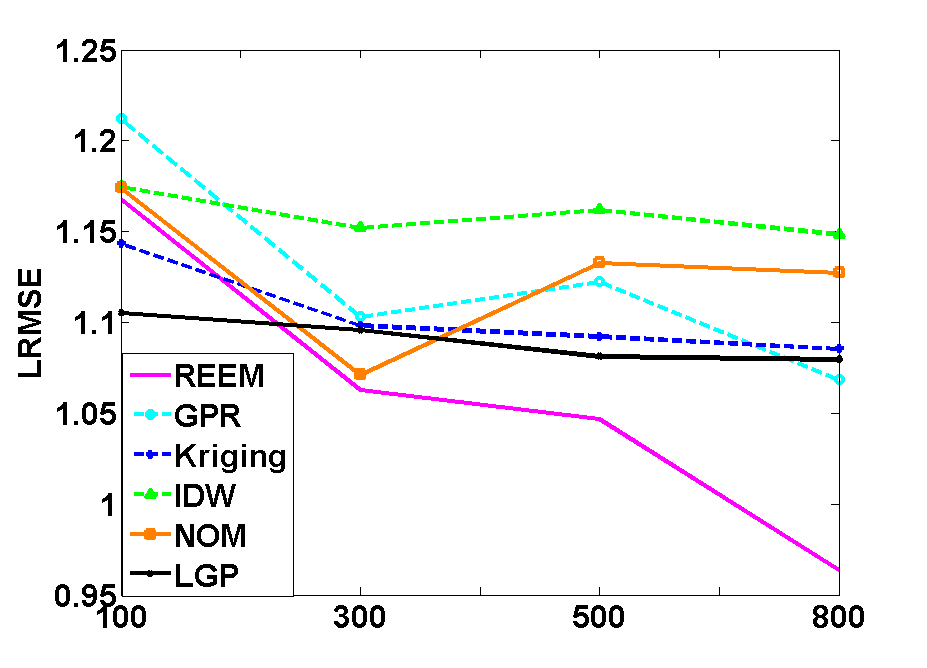
\includegraphics[width=0.72\linewidth]{pictures/performance.png}
%}
%\caption{\label{fig:performance}The LRMSE of evaluation on different training points(100, 300, 500, 800 data points, respectively)}
%\end{figure}
%
\subsection{Time Cost Comparison}
%As to real-time model, time cost, usually consisting of training cost and estimating cost, is a crucial criterion. Since LGP and IDW are online training model, Fig.\ref{fig:trainingtime} just illustrates the training time comparison among OEEM, GPR and Kriging, where we can see our model have obvious advantages. Besides, considering the average time in millisecond needed for estimation of 1 query point shown in Table\ref{tab:testingtime}, OEEM outperforms standard GPR, LGP and Kriging while being close to IDW.
%\begin{figure}[!htb]
%\centerline{
%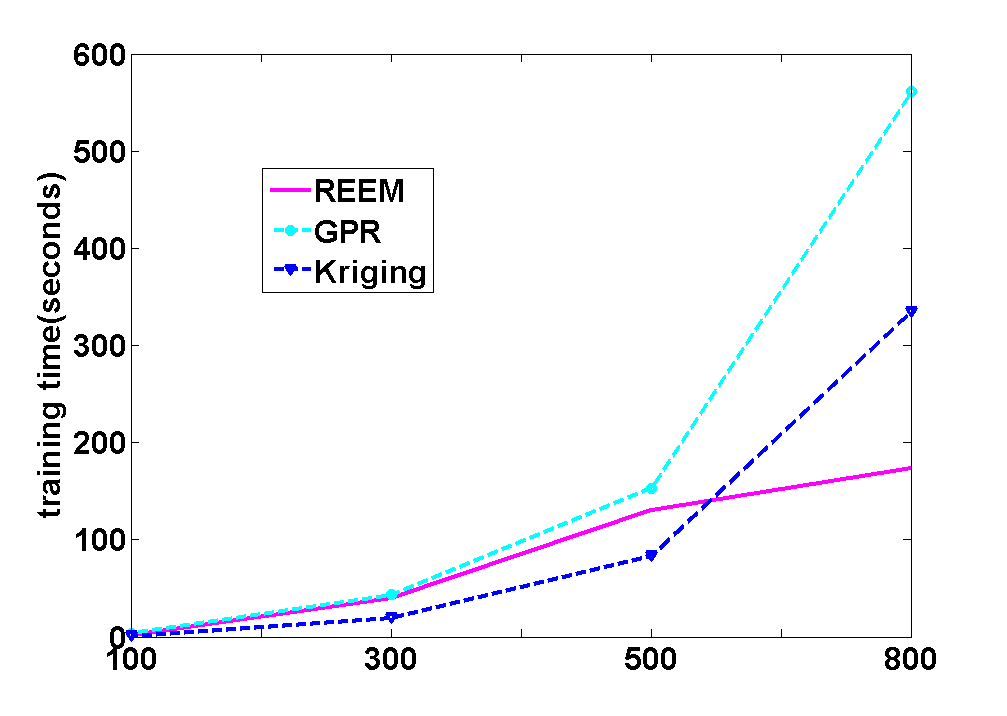
\includegraphics[width=0.72\linewidth]{pictures/trainingtime.png}
%}
%\caption{\label{fig:trainingtime}The comparison of training time on different datasets with decreasing training points}
%\end{figure}
%
%\begin{table}[!ht]
%\footnotesize
%\caption{The comparison of average time needed for estimation of 1 query location on different models}
%\label{tab:testingtime}
%\def\tabblank{\hspace*{10mm}}
%\renewcommand{\multirowsetup}{\centering}
%\begin{tabularx}{0.5\textwidth}
%{@{\tabblank}@{\extracolsep{\fill}}lccp{100mm}@{\tabblank}}
%\toprule
%  model & querying time(millisecond) \\\hline
%  REEM & 0.31 \\
%  standard GPR & 0.73 \\
%  LGP & 73.39 \\
%  Kriging & 0.47 \\
%  IDW & 0.22 \\
%\bottomrule
%\end{tabularx}
%\end{table}
%
%In conclusion, comprehensively considering the performance of accuracy and time, our model is the best-performing model.
\section{Conclusion and Future Work}
Our goal is to do real-time urban air quality estimation with mobile sensors system. We proposed and implemented Real-time Ensemble Estimation Model (REEM) based on GPR. We evaluated the model with mobile data from mobile sensors system located in Beijing. The experiments showed our model outperforms other state-of-art models both on precision and time efficiency.

The next works we can do to improve the air quality estimation are as follows:

The diffusion of pollutants in the air is sophisticated influenced by many different factors. Inspired by the Land-Use Regression, we can integrate the city's POI information into our model. Besides, the spatio-temporal distribution of sampling positions depends on the current positions of vehicles with the sensor randomly. Thus, we can design an algorithm for route planning in order to optimize the spatial-temporal distribution of observations. Actually, as for the air quality data from mobile sensors, there is a problem need to be solved. Since the mobile sensor located on the car is close to pollution source, the pollution level of monitoring data is higher than that of the truth. Based on supervised learning, we should try to design an algorithm to correct the observations from vehicles with static monitoring stations.

With the rapid development of mobile sensors, how to take full advantage of mobile data is a meaningful and challenging task.
% References and End of Paper

\bibliography{AQE_draft}
\end{document}
% end of Itexpprt.tex
